%%
%% Author: shoupu_wan
%% 7/14/18
%%

\chapter{Strive for Lean Loops} \label{ch:loops}

As one of the most widely used programming constructs, loop is productivity
amplifier and is featured in almost all programming languages.
With a static body and nominal overheads (\textit{e.g.},
state-registering variables, \textit{etc.}), a loop can be executed as many times as desired.


A key building block as loop is, it is worth every developer's effort to master the best
practices of it.
On the opposite, it is not uncommon to spot in production code, especially algorithm-intensive code
haphazardly constructed loops, often with duplicate code dangling around.
Obviously developers who authored the haphazardly `working' code were either oblivious
with good programming practices or does not bother to spend the time on better loop constructs.
%Have you deliberately tried out a few loop constructs and chosen the best fit for a specific
%application?
%I wish your answer to these questions are both positive.
%This is so not because these developers have no appetite for better code.


For this reason I would like to devote a substantial part of this book to clarify the best practices
concerning the construction of loops.
The major focus of this chapter is `How to avoid duplicate code?' and
`How to fix up slack loops?'
Slack loops refer to quick-n-dirty loops with duplicate code in and around it.
We will elaborate on techniques that can help one construct `lean loops'.
Once the habit of coding `lean' is formed, one will automatically, proactively seek to author high
quality code.
%``How to tighten up slack loops''.


Another topic of this chapter is ``how to limit the scope of loop variables?''
Have you experienced that a leaky and long living loop variable is the root cause of a malicious
bug?
I am positive you are not unfamiliar with this.
Inadvertent namespace contamination often houses the most treacherous bugs.
Loop variables at large is a common cause for namespace contamination.
So when we program loops, we need to pay attention to running away loop variables.


A related topic is on the use of nested loops.
Nested loops are often a sign of suboptimal code in many circumstances.
Therefore `how not to use nested loops' is critical to reduce clutters out of one's code.
We dedicate ~\fullref{ch:embedded-loops} solely to this topic and presents techniques to help
reduce nested loops to single loop.


\section{Loop anatomy}\label{sec:loopAnatomy}

%For completeness, a summary of
%later discussions of the interactions between conditional statements and loop is built on
%top of reader's mastery of loop programming.
%As in ~\fullref{ch:organizeYourIfElse}, most of the techniques presented in this chapter are
%first-hand, based on the author's own coding experience.
%But most importantly, I intend this chapter can inspire enterprising
%programmers to habitually reflect on their code and discover new ways to improve.

Here we will give a brief account of the parts of a loop.
We do so in a generic sense with several mainstream programming languages in mind.
First off, entering a loop is like entering a building---before one proceeds, one needs to know
where the exits are or infinite loop may result inadvertently.
For this reason, all loop constructs come with a termination test.
The location of termination test is a distinguishing feature for a loop.
Based on its location, loop constructs can be classified as \emph{pre-test}, \emph{post-test},
and somewhere in between, \emph{mid-test}.
post-test loops attempt to execute the loop body at least once no matter what.
Mid-test loops may execute part of the loop body.


Secondly, most loops have initialization sections for preparatory work.
%Initialization rightly takes some deliberation as it is coupled with the loop body.
Thirdly, as a finite-state machine, a loop construct necessarily has state updating statements
which push the loop toward its termination.
Finally there is so-called `post-loop processing', one-off processing immediately after a loop
terminates.
%under certain circumstances, may be assimilated into the loop.


\begin{table}[htb]
    \begin{center}
        \caption{Loop anatomy\label{tbl:loop-construct}}
        \begin{tabular}{l|p{10cm}}
            \hline
            Component & Description \\
            \hline
            \emph{Loop initialization} &
            This is the preparatory section before the execution of a loop.
            For \code{while}-loop, this is done outside of the loop.
            In \code{for}-loop, this may be done in the \code{<init>} section of the
            \code{for}-loop construct or both.\\
            \emph{Loop test or loop condition} &
            The condition for control to enter (or continue) the loop. \\
            \emph{Loop body} &
            The block of statements to be executed in the loop. \\
            \emph{Loop state updating statements} & Almost all loops come with stateful loop
            variables.
            Updating the loop variables are important job of the loop.\\
            \emph{\code{break} statement} &
            A statement in loop body that breaks the loop and pass control to the next statement
            following the loop. \\
            \emph{\code{continue} statement} &
            A statement in loop body that interrupt the execution of the remaining
            statements in the loop.
            Note that this doesn't break the loop or pass control out of the loop. \\
            \emph{\code{return}, \code{yield}, \textit{etc.}} & These statements are
            not part of the loop construct yet they affect the control flow of the loop. \\
            \emph{Post-loop processing} &
            These are rare loop constructs, such as \code{while..else} and \code{for..else}
            in \python. \\
            \hline
        \end{tabular}
    \end{center}
\end{table}


~\autoref{tbl:loop-construct} summarizes the common parts in loop constructs of most high-level
programming languages.
On top of the standard loop constructs, possible customizations may be made with \code{break},
\code{continue}, \code{return}, \textit{etc.}, depending on the programming language of choice.
These statements blend into the loop body and fine tune the execution paths of otherwise standard
loops.


Many programming languages conveniently support more than one types of loop constructs.
\code{for}-loop and \code{while}-loop are examples of pre-test loop constructs that
almost all languages support.
\code{do-while}-loop is a post-test loop construct supported by \java, \cpp, C, and many
others (excluding \python).


Why do we need these many varieties of parts and loop constructs?
Let us illustrate the abstract concepts with concrete examples.
Say, in a cooking contest, each chef is to cook 3 dishes in a course---appetizer, main,
and desert.
Interested judges will approach the team and put an order of a full course.
Other than judge orders, chef does not cook anything else.
The competition process may be best coded with pre-test loop such as
\lstinputlisting{loop/pre_test_loop.java}


Suppose, on the last night of the competition, the rule is changed so that each chef is to cook a
course for display before judges' orders.
One can do a `copy-n-paste' to solve the problem;
or one can avoid `copy-n-paste' with a post-test loop:
\lstinputlisting{loop/post_test_loop.java}


For another example, suppose we are to develop a command line tool that takes input from
\code{stdin}.
The tool interprets user input and does a bunch of cool stuff.
It terminates when user types `exit' or simply hits `return' key
(in which case the input string is empty).
Then the best loop construct for that would be mid-test loop.
But since \java does not have a specialized mid-test loop construct, we have to makeshift by using
a \code{break} statement along with an infinite loop:
\lstinputlisting{loop/mid_test_loop.java}


\section{A word on the usage of \code{continue}, \code{break}, and \code{return}}
\label{sec:continue-and-break}

We have touched the topic in ~\fullref{sec:branchinginloop} of ~\fullref{ch:organizeYourIfElse}.
For most cases, where \code{continue} statement is used may be
equivalently realized by adding an \code{else}-clause.
But when used in a `cascading conditional' (see ~\fullref{ch:conditional-cascade}),
`\code{continue}' can simplify the loop body like a magic.
Earlier in ~\fullref{ch:organizeYourIfElse}, we illustrated the use of \code{continue} statement in
`Zoo animal health exams' problem.
At the risk of repetition, I am going to provide yet another example if only this can inspire the
reader to strive for optimal loop construction.
Suppose we are coding a game for two or more players with the following rules:
\begin{enumerate}
    \item All players take turn to enumerate natural numbers starting from $1$;
    \item When the number is divisible by $2$, the player write the number down then claps their
    hands;
    \item Otherwise when the number is divisible by $3$, the player write the number down then
    stump their feet;
    \item Otherwise when the number is divisible by $5$, the player do nothing;
    \item Otherwise the player write down the number and articulate the number loudly.
\end{enumerate}
These rules are applied in the order as they appear.
Namely, a `$10$' is not be skipped;
neither is `$15$';
but `$25$' is.

How would one solve the problem?
Without `\code{continue}', there are two obvious choices---either use composite tests such as
`\code{n \% 5 and not n \% 2 and not n \% 3}; or use nested conditionals.
Interested readers may try this on their own.
For the first choice, it involves redundant tests.
Suppose an additional rule regarding `$7$' is added, then the places to change would be doubled.
For the second choice, the readability would be compromised with the `switching
smell'\cite{Fowler1999}.
Even worse, duplicate code may chip in by repeatedly invoking `\code{result.append(i)}' for the
cases of `$2$' and `$3$', respectively.


Thankfully, an implementation using `\code{continue}' statement in conjunction
with a cascade conditional is free from any of the problems listed above:
\lstinputlisting{loop/use_of_continue.py}
It is marvelous!

%TODO settle down this presentation
%% side-by-side two columns
%\begin{clisting}
%    \begin{minipage}[t]{.45\textwidth}
%        \lstinputlisting[caption={Using \code{if-else}.}]
%        {loop/conditional_in_loop_no_continue.java}
%    \end{minipage}\hfill
%    \begin{minipage}[t]{.45\textwidth}
%        \lstinputlisting[caption={Using \code{if..continue}.}]
%        {loop/conditional_in_loop_continue.java}
%    \end{minipage}
%\end{clisting}

% side-by-side two columns
%\begin{clisting}
%    \begin{minipage}[t]{.45\textwidth}
%        \lstinputlisting[caption={Unsimplified code}]
%        {loop/loop_cond_redundant_testing.java}
%    \end{minipage}\hfill
%    \begin{minipage}[t]{.45\textwidth}
%        \lstinputlisting[caption={Simplified code}]
%        {loop/loop_cond_repeated_block.java}
%    \end{minipage}
%\end{clisting}
%But each has their own problem.
%The left column do redundant condition testing (test1), whereas the right column has repeated
%code (\code{statement2}).

%The simplification of both lies in the use of \code{continue}:
%
%\begin{minipage}[H]{\textwidth}
%    \lstinputlisting{loop/loop_cond_no_redundancy.java}
%\end{minipage}


Similar situations may exist for the use of \code{break}, \code{return}, \textit{etc.} to reduce
redundant code.


\section{C-style For-loop}\label{sec:for-loop}

Beside the universal \code{while}-loop, is the conventional C-like \code{for}-loop
\footnote{This is not to be confused with the iterator-based \code{foreach},
whose functionalities has largely been replaced by streaming such as in JDK 8+.},
another commonly used pre-test loop whose layout looks like looks like
\lstinputlisting{loop/for_loop.java}
The distinguishing parts of a \code{for}-loop are its header statements---the
initialization \code{<init>}, the loop test \code{<test>}, and the afterthought \code{<aftrth>}.
Below is an explanation of these header statements:
\begin{enumerate}
    \item The \code{<init>} is a statement to be executed only once as control is transferred to
    the loop.
    \item The \code{<test>} may be regarded as the \emph{first} statement of the loop body.
    \item The \code{<test>} are executed one more time than the rest of loop body
    unless loop execution is aborted with, say, \code{break}.
    \item The \code{<aftrtht>} is the afterthought statement executed at the end of each
    iteration of loop body even in the presence of \code{continue}.
    But in the presence of \code{break} statement, \code{<aftrtht>} will be skipped together with
    part of the loop body.
    \item All three header statements are optional.
    Namely, `\code{for(;;);'} is perfectly legal and represents an infinite loop.
\end{enumerate}


Design considerations for a \code{for}-loop are generally related to the header statements.
Where to update loop state?
For example, where should \code{i++} or \code{j--} be placed?
In the afterthought header or somewhere in the loop body?
How to arrange terminating statements?
Should the loop test header statement be used or use an `\code{break}' statement in the body?


All these considerations are tightly coupled and changing one will likely result in changing all.
For example it is more flexible (sometimes necessary when certain condition
has to be met to increment/decrement)
to increment/decrement state variables in loop body but it may not be the most concise form.
In a more concise loop, state updates are often done in the afterthought header statement.
For another, infinite loop is often the result of a reasoning loophole,
which causes incorrect termination condition.


To me personally, the single biggest reason to use a \code{for}-loop is its limited scope of
loop variables declared in the \code{<init>} header statements---they are invisible beyond the loop.
For example the following code wouldn't compile
\begin{lstlisting}
    for (int i = 0; i < 10; ++i) {}
    System.out.println(i); // i is undefined
\end{lstlisting}
In contrast, loop variables used by the \code{while}-loop condition have to be declared
before the loop.
Therefore they leak beyond the loop.


%Occasionally limited scope of \code{for}-loop may be a hinder for post-loop processing.
%If that is the case, one may resort to
%`one-more-cycle' technique (see ~\autoref{sec:one-more-cycle} for more details) to solve the
%problem.
%Also for \python users, \code{for-else} or \code{while-else} is designed just for post-processing.


\section{Refactoring loops}\label{sec:refactoringLoops}

Many loops, especially those embedded in a crammed function, should be
refactored into a function just containing the loop and minimal post-loop processing logic.
Doing so not only makes the logic stand out in the original function,
but also the factored out function is compact, single-purposed, and reusable.

To eliminate of intermediate, local variables is another reason for refactoring loops into a
dedicated function.
Intermediate variables in a long function often share the same scope as the function
and thus contaminate the namespace in the latter part of the function.
Please by all means do yourself a favor and eliminate long-standing intermediate variables.
This simple thumb rule will help prevent mysterious bugs and spare you from ghost-chasing.


The following example illustrates this.
In the first version, the code in the main function \code{execute} was
misappropriated---a large part of it was usurped by the loop whose sole purpose
is to search for `a needle in the haystack'.
\lstinputlisting[lastline=12]{loop/refactor_conditional_in_loop.java}
In the following listing, we refactored the loop into a separate function.
Not only did we greatly reduced the bulging function, but most importantly
\code{target} and other intermediate variables are eliminated and
their scope are caged in the new function.
The threat of polluting the namespace in the remaining code is completely removed.
\lstinputlisting[firstline=14]{loop/refactor_conditional_in_loop.java}


\section{The `\textit{loop-and-a-half}' problem}\label{sec:loop-and-a-half-Problem}

As discussed above, when it comes to programming with loops, there are a variety of constructs
such as pre-test loop and post-test loop.
Have you wondered why we need so many varieties and families?
Is there a one-size-fit-all loop?


To answer this question, let's dig into history a bit.
In 1966, Corrado B\"{o}hm and Giuseppe Jacopini proved that \code{goto} statements are
unnecessary and programs containing them can be transformed to use only conditional statements
and loops\cite{Bohm:1966}.
Along that line of thinking, more researchers, who might have gone too far, attempted to remove
other `nuisance' in computer programming such as \code{break} and \code{return} in the middle of a
loop to reduce control flow complexity and promote code composability.
But the benefit for doing so does not pay for itself---one ends up with having to create more
intermediate variables.
one result of doing so is that more local variables are needed.
Even worse, it exacerbates problems with duplicate code in and around a loop.
This is the origin of the so-called ``Loop and a half problem''\cite{Louden-Lambert-2011}.
Today, ``\textit{loop-and-a-half} problem'' is still a pestering problem for suboptimal loop
design and implementation.


At the language level, a number of loop constructs have been introduced to
minimize the symptoms of the ``\textit{loop-and-a-half} problem''.
But that's not enough.
The burden remains with developers to choose the most suitable loop constructs.
Further, code fine-tuning is beyond simple choices of loop constructs
and must be hand-crafted at implementation time.
In the section to follow, we will introduce `loop rotation', a technique for loop
optimization that helps alleviate `loop-and-a-half' symptoms.


It may be unexpected to many.
But sentinels can also be used to cure `loop-and-a-half' problem.
We will study a few cases for this in ~\fullref{ch:sentinels} and in
~\fullref{ch:json-prettifier}.


\section{Loop Rotation}\label{sec:LoopDesignConsideration}
\begin{figure}[htb]
    \centering
    
\includegraphics[width=.7\textwidth]{loop/ferris-wheel.jpg}
    \caption{\label{fig:loop-rotation}Loop as a circular sequence.
    The nodes \code{i++} and \code{print} are candidates that can matched and coalesced into
    the loop.}
\end{figure}


Why programming loops is so hard?
For one, there are a lot of moving parts in a loop construct and need to be constructed
piece-by-piece.
For two, loop must get along with the peripheral code as well.
As you can see, a large part of the hard work for programming a loop lies outside of the loop.
All the pieces are tightly coupled together---changes in one necessitate changes in several others.


In fact, an important goal when implementing loops is to reduce duplicate code in and around
loop---be it pre-loop initialization or post-loop processing.
And one of the important techniques for it is `loop rotation'.


It is beneficial to visualize a loop construct as a Ferris wheel, a carousel, or a spool.
Mathematically speaking, a property is shared by all four---they all represent circular sequences, that is,
a sequence with rotational symmetry with respect to circular shifts.


If pictured as a Ferris wheel, distributed around the wheel are the conditional test,
initialization, state update statements and other statements in the loop body.
(see ~\autoref{fig:loop-rotation}).


\begin{figure}[htb]
    \centering
    \begin{subfigure}{.45\textwidth}
        
\includegraphics[width=\textwidth]{loop/loose-spool.jpg}
        \caption{\label{fig:loose-spool}}
    \end{subfigure}
    \begin{subfigure}{.45\textwidth}
        
\includegraphics[width=\textwidth]{loop/tight-spool.jpg}
        \caption{\label{fig:tight-spool}}
    \end{subfigure}
    \caption{\label{fig:spool-loop} If we use spool as a metaphor for loop in program, then
    `loop rotation' can be pictorially depicted as winding up loose yarns onto a spool.
    \protect\subref{fig:loose-spool}: Duplicate, sloppy code is analogous to loose, unorganized
    yarn around a spool.
    \protect\subref{fig:tight-spool}: A neat loop is analogous to a tidy spool.}
\end{figure}


Circular sequence may be cut open and mapped to a linear sequence, \textit{e.g.}, starting with
the lowest node going counterclockwise.
As if a ring may be cut open, the nodes in a circular sequence may be ordered as a linear sequence
if counting counterclockwise starting with the lowest node.
One thus may take advantage of this rotational degrees of freedom as a measure of loop fine
tuning---by `rotating' the loop to match up and coalesce duplicate code in the affinity of the loop.
We will refer to this process as `loop rotation'.


As another helpful analogy, loops are to program as spools are to yarn.
In the same way as a spool is used to organize yarn, a loop is a construct to organize program.
From this perspective, the `loop rotation' process to coalesce duplicate code is analogous to
wind up loose, messy yarn into a tidy spool (~\autoref{fig:spool-loop}).


In practice, one may first implement a prototype with unconditional \code{while (true)} or
\code{for (; ;)} loop.
This will push all the statements into the loop body for ease of `loop rotation'.
In this way, one first focuses on coming up with a working solution.
Once a working solution has been found, one can start the `loop rotation' process.
%one often has gotten a good grasp of the ins and outs of the implementation.
%to to try to spool up slack threads as much as possible by `rotating the loop' to match and
%eliminate duplicate code.
Finally, one can try different loop constructs, move and fit state-updating statements,
combine or annihilate \code{continue} and \code{break} statements, \textit{etc.}
If needed, repeat the above steps until the code is acceptable both functionally and
aesthetically.


Let us take a look at a toy example at which the `loop rotation' process can be easily applied.
It is the driving function: it creates the players, the board, the pieces, then it passes
control to the main loop, at end of the game, it presents the final result.
So here we go, the code to be improved is listed below.
\begin{clisting}[H]
    \lstinputlisting[]{loop/board_game_dupcode.py}
\end{clisting}
Looking at , as we rotate the loop, they can be aligned and coalesced line by line.
As can been seen, the last statement in the loop and the immediate statement before the loop
(lines $2$-$5$ and lines $18$-$21$ as highlighted)
are verbatim duplicate and thus may be aligned and coalesced.
So we can `roll up' the immediate statements before the loop and coalesce them with their
counterparts in the loop body.
But first of all, we need to untie the loop by `internalizing' the loop condition
so that it becomes an unconditional `\code{while(True)}' loop:
\begin{clisting}[H]
    \lstinputlisting[]{loop/board_game_dupcode-0.py}
\end{clisting}
Now watch closely---let us roll up one line:
\begin{clisting}[H]
    \lstinputlisting[]{loop/board_game_dupcode-1.py}
\end{clisting}
As you noticed, we have aligned and coalesced one line of the duplicate code.
Repeating this process $4$ more times, we would wipe out all duplicate code.
The final program looks like the following:
\begin{clisting}[H]
    \lstinputlisting[]{loop/board_game_rotated.py}
\end{clisting}
In practice you don't have to strictly go through each and every step described here.
Once you grasp the idea and become skillful, you can skip some of the intermediate steps
to quicken the process.
And you can always find your way back if you are lost.


Many times, code duplication are `soft'---two or more blocks of code are not exactly
identical but contains identical snippets or share common pattern.
We will refer to this type of hidden, quavery, and partially duplicate code as
`soft duplication'.
In contrast, we may refer to copy-n-paste code as `hard duplication'.
Comparing with hard duplication, soft duplication is tougher to detect and remove.
When dealing with soft duplication, one may perform pre-refactor to
consolidate soft duplications into hard ones and then deal with hard duplication in the normal way.


\section{Loop Initialization}\label{sec:loopInitialization}

Initialization is the preparatory code for a loop.
%Initialization and the loop body each has its focus.
It is a preclude, a bridge to the loop body.
Initialization can also be deemed as a `primer coating' that prepares a substrate for the loop
body to deposit changes iteratively.


A proper initialization lays the foundation of success of the loop implementation.
A simple initialization helps reduce explicit and hidden code duplication.
More often than not, loop initialization takes simple, effortless,
intuitive values---integer $0$, empty list, zero-length string, array of simple values,
\textit{etc}.
But occasionally, initialization \code{int i = -1} may have an edge over \code{int i = 0}.
This requires one to push the boundary to achieve a simpler initialization.


As another brief example, when people think about Fibonacci sequence, they usually think it starts
with $1$:
\begin{table}[H]
    \centering
    \begin{tabular}{c|c|c|c|c|c}
        \hline
        $i$ & 1 & 2 & 3 & 4 & \ldots \\
        \hline
        $f(i)$ & 1 & 1 & 2 & 3 & \ldots \\
        \hline
    \end{tabular}
\end{table}
But add a zeroth-element to Fibonacci sequence sometimes opens new ways of thinking.
\begin{table}[H]
    \centering
    \begin{tabular}{c|c|c|c|c|c|c}
        \hline
        $i$ & 0 & 1 & 2 & 3 & 4 & \ldots \\
        \hline
        $f(i)$ & 0 & 1 & 1 & 2 & 3 & \ldots \\
        \hline
    \end{tabular}
\end{table}
Similarly, when it comes to factorial, many people starts with $1!=1$, seldom $0!=1$.
But the latter is a critical step toward the analytic expansion of the domain of factorial
functions to complex domain, in which it is known as the $\Gamma$-function.


You will see more cases later where generalization of the algorithm and/or the mathematical
concept will make the coding, and particularly initialization, easier.
Simplifying initialization process is especially important for dynamic programming.
Interested readers may skip to ~\autoref{ch:dp} to look for more information.
As in the `spiral termination' problem, sometimes looking for more general mathematical forms
means backing off from the most `intuitive' initialization and this mindset may get you in another
level of code proficiency.


In light of the `loop rotation' technique, in some cases one can take advantage of the rotational
degree of freedom of a loop to coalesce duplicate initialization
or post-loop processing code into the loop.
If you find that your initialization code actually repeats the loop body in whole or in part,
or that the post-processing logic does similar things as the loop does,
that's a sign that you should `tighten' your loop.


Loop initialization should be trivial and light-weight.
Apart from being correct, initialization should also be small.
%Let each maintain its focus---a minimal, light-weight initialization focus on the preparatory work
On the other hand by design, loop body does the heavy lifting---it is responsible to progressively
mutate the initialized state to the desired final state.


Pretty simple, isn't it?
It depends.
For one who has formed a habit of striving for the simplest,
this requirement for initialization seems intuitive and natural.
But for one who is new to this, it may be a struggle
to figure out what is the correct and minimal initialization.
For example, should the initialization be \code{int i = -1} or \code{int i = 0}?


Let us take a look at the 'spiral termination problem':
\begin{quote}
    Given the dimensions of a $2$D matrix, $m$ and $n$,
    one is to visit each and every cell of the matrix in
    a clock-wise, spiral fashion from the upper left corner.
    Determine the final position when the visit finishes.
    For example, when $m=1,n=1$, it is $[0,0]$.
\end{quote}


There are more than one solutions to this problem---both iterative and recursive.
We are here to demonstrate an iterative solution with a loop.
Note that since the problem only asks for the final position,
cells passed by along the way are irrelevant.
As such, we can `hop' over cells.
Without making too much a pitch, here is an outline of the algorithm we are to implement:
\begin{quote}
    Approach the termination position in `strides'.
    In each stride, we hop over a perimetric layer of cells.
    A `perimetric layer' here consists of all the cells not yet visited but not completely
    surrounded by unvisited neighbors (see ~\autoref{fig:spiral-term-iter}).
\end{quote}


In general, if we start off at $[i,j]$ and after we finish visiting a perimetric layer,
we will finish at $[i+1,j+1]$ as shown in ~\autoref{fig:spiral-term-iter}.
\ldots Albeit for special cases when the matrix is an array (columnar or row alike).
In that case, the terminating cell is at end of the line.
For now, we are going to handle this extra complication with post-loop processing.
Altogether, apart from the to-be-determined initialization and post-loop calculation, the main loop
looks like
\lstinputlisting[]{loop/spiral_termination_todo.py}
Now all stake is laid on the initialization.
As long as that can be determined, the rest of the
code will bring it where need be.
``But what is the starting point?''


\begin{figure}[tbh]
    \centering
    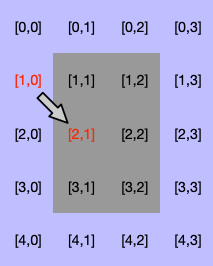
\includegraphics[width=.4\textwidth]{loop/spiral-term.jpg}
    \caption{\label{fig:spiral-term-iter}
    Iteration after one `spiral stride' in the `Spiral termination' problem.
    Purple cells denote a visited `layer'.
    Cells in red are the final positions after the first and second iterations, respectively.
    The arrow represents the final displacement from the end of first iteration
    to the end of the second.}
\end{figure}


At the first glance, initializing $i=j=0$ seems reasonable.
For example, when $m=n=3$, after `peeling off' the outer layer, \code{i,j} becomes
$[1,1]$ and indeed the process terminates on $[1,1]$.
However we will encounter problem for case $m=n=2$, for after the outer layer, our program would
end up on a eerie, non-existent cell $[1,1]$.
(The correct answer should be $[1,0]$.)

In retrospect, we are somehow one-step too further in each iteration.
This will be a problem whenever \code{min(m, n)} is an even number.
To make this work, one remedial measure is to abstain from the last iteration---it is the very
iteration that throws us off the cliff.
This is essentially applying the reverse process of `one-more iteration'
We can thus refer to this process as `one-less-iteration'.
Convince yourself that by doing so, this condition `\code{1 <= min(m, n) <= 2}' will hold true
upon loop termination and the leftover is handled in post-loop processing.
With this fix, here comes the first complete solution that works:
\lstinputlisting[]{loop/spiral_termination_final.py}
In this solution, the initialization is natural and trivial.
But still the loop condition `\code{2 < m and 2 < n}' seems little unintuitive and arbitrary.
After all, why `$2$'?


Keep in mind that this is not the only solution.
Far less so is it the best.
An straightforward thought to the `one-step-too-further' issue is ``Why not take a step back?''
Let us take a step back, literally.
%Let us step back from initializing \code{i, j = (0, 0)}.
Instead of thinking in terms of `the first cell of the next iteration', let us think in terms of
`the last cell in the previous iteration'.
With that mindset shift, we can flip our perspective from initializing the `starting point'
to the `finishing point'.
In other words, let \code{i, j} represents the finishing point.
For example,  $[1,0]$ is one of `the last cells of iterations' in ~\autoref{fig:spiral-term-iter}.


But the new problem is, ``Without an iteration in the first place, how do we get `the last cell of
previous iteration'?''
As a matter of fact, for a big enough matrix, [1,0] is always `the last cell of an iteration'.
But for edge cases where the matrix is not big enough, we could directly calculate and return the
result without ever hitting the loop.
So presumably, conditional statement is needed before the loop to distinguish different cases.
But keep in mind that the same logic will be needed again in post-loop logic.
Therefore if we initialize \code{i,j = 1,0}, duplicate code would be inevitable, one way or the
other.
%You may notice that the code before and after the loop deals with similar scenarios, shares
%commonality, and thus are inevitably duplicate to some degree.
%How to get rid of the duplicate code before and after the loop?
How to proceed from here?


\begin{figure}[tbh]
    \centering
    
\includegraphics[width=.4\textwidth]{loop/spiral-term-init.png}
    \caption{\label{fig:spiral-term-init}
    `Spiral termination' problem: backtracking the initialization to an extrapolated,
    virtual cell.}
\end{figure}


At the same time, another haunting question is ``What should be returned for a $0$-sized
matrix?''
The key for both these questions lies in `backtracking' the initialization.
As shown in ~\autoref{fig:spiral-term-init}, if we extrapolate the path backwards, we would end
up on a serendipitous, virtual cell that is not part of the matrix.
Its value is, obviously, `[0,-1]'.
Should we initialize \code{i, j} to `$[0,-1]$'?


Now the situation becomes a little bit too philosophical.
%This value still aligns well with our `Be small' requirement for loop
%initialization.
%The `path' taken by the loop, the stops after each iteration of the loop give us a hint.
%As in ~\autoref{fig:spiral-term-init}, if we extrapolate the path backwards
%(in the opposite direction to the arrows), we  discover the cell `$[0,-1]$'.
On the one hand, it sounds crazy to initialize the loop variables to an invalid cell, that is not
part of any matrix.
On the other, a closer examination reveals that the virtual cell not only serves as a perfect
`sentinel' for the case of $0$-sized matrix,
in the same way as \code{null}  for the `lack of an \code{Object}',
but also makes a good initialization value that will lead to correct result and aligns well with
`Be small' requirement.
%So `$[0,-1]$' can be deemed as the sentinel value for zero-sized matrix.
More importantly, it is the key to get rid of the duplicate code.


Without much ado, here is the iterative solution with the newly discovered initialization key:
\lstinputlisting[]{loop/spiral_termination_virtual_init.py}
This solution has an advantage over the previous in that
its input domain is larger than other---it can handle zero-sized matrices while its predecessor
cannot.
This is analogous to concept of `analytic continuation' in complex analysis if
reader is familiar with the topic.


As can be seen, changing the initialization from [0,0] to [0,-1] in between the above two solutions
is a big deal to the program.
As a result, the whole programming scenario is changed---the loop condition is changed,
the post-loop processing logic is changed.
This again explains why it is so hard to refactor a loop---the stake of inadvertently changing
its behavior or correctness is very high.


Through the `spiral termination' problem, we see that initialization plays a key role in loop
implementation.


Before we conclude this section, I want to let you know that there is a 3-liner solution to the
`spiral termination' problem:
\lstinputlisting[]{loop/spiral_termination_two_liner.py}
Or may be even simpler solutions that I don't know.
By telling you this 3-line spoiler, I am not at all telling you that your
optimization effort so far has been totally wasted.
Far from it, the information I want to convey is ``Something is built to be thrown away
at due time.''
Until that time comes, everything that exists and optimization efforts thereof are
meaningful and have their intrinsic value.


\section{Dedupe Post-loop Processing}\label{sec:one-more-cycle}

It is normal that after loop termination, non-trivial post-loop logic is needed to
transform the output to final form.
But if one finds that the post-loop code repeats certain statements in the loop body,
that is an alarm calling for code deduplication.
But if one finds that the post-loop code shares similar functionalities,
repeat certain steps in part or in whole with the loop body, one should sound the alarm.
A technique to be explained below may help you.


This technique, named `one-more-cycle', changes the loop-termination condition so that
the number of iterations in the loop is extended by one, the loop body is executed \emph{one more time}
than otherwise.
More often than not, extra logic in the loop body is needed to handle the extra iteration
slightly differently.
This is especially true if it is only soft duplication.


Again, let me illustrate the whole process with a real example.
What we will study here is the `Maximum rectangular area under
histogram' problem (problem statement is available on several sources, \textit{e.g.},
GeeksforGeeks\footnote{\url{https://leetcode.com/problems/largest-rectangle-in-histogram}}
or LeetCode\footnote{\url{https://www.geeksforgeeks.org/largest-rectangle-under-histogram}}).

The optimal algorithm for this problem is the one using an auxiliary \code{Stack<Integer>}.
For a detailed discussion of the algorithm, refer to the above mentioned sources.
Here is a brief summary of it (suppose input is an array of integers \code{heights}):
\begin{alisting}[H]
    \caption{\label{enum:stack-limited-mining-algo}Stack-based algorithm for
    the `maximum rectangular area under histogram' problem}
    \begin{enumerate}
        \item Initialize an empty \code{stack}, the whole purpose of
        which is to store indexes of an ascending subsequence of heights.
        \item Store a progressive max result initialized as \code{maxRec=0};
        \item For each \code{(index, height)} in the histogram
        \begin{enumerate}
            \item Pop all the indexes on \code{stack} whose corresponding heights are
            $\geq \mbox{\code{height}}$
            \item For each popped index \code{i}, update \code{maxRec} with the
            rectangular area formed between $[\mbox{\code{top}}, \mbox{\code{index}}]$
            with a height of \code{heights[i]}, where \code{top} is top of \code{stack}.
            (Watch out for boundary cases!) \label{itm:pop-update-maxRec}
            \item Push \code{index} onto \code{stack}.
        \end{enumerate}
        \item For each remaining index in \code{stack}, do the calculation
        as ~\ref{itm:pop-update-maxRec}, replace \code{index} with length of input array.
        \item Return \code{maxRec} as the final result.
    \end{enumerate}
\end{alisting}


Based on a random sample of submissions on LeetCode, majority of the implementations
of ~\autoref{enum:stack-limited-mining-algo} are more or less like what follows:
\lstinputlisting[]{loop/histogram_verbose.java}
While it passes $100\%$ the unit tests and was accepted by the Online Judge, this
solution has various smells.
The smelliest issue is the oversize post-process code, the entire \code{while}-loop which
is almost a verbatim repetition of the body of previous loop.
If we can get rid of this code duplication, the code quality would be greatly boosted.


The `one-more-cycle' technique is invented just for this.
Let us explain how it works.
First, extend the number of iterations in \code{for}-loop by one---instead of the loop
condition `\code{i < heights.length}', use `\code{i <= heights.length}'.
The second step is to delete the post-process \code{while}-loop.


The code as it is now does not work.
Why?
It throws `\code{ArrayIndexOutOfBoundsException}' for there is no such an element as
`\code{heights[heights.length]}'.
Once identified, it's an easy fix---we just need `extra logic' to shield
the code `\code{heights[i]}'


Shown below in ~\autoref{lst:histogram-oneMoreCycle} is
a refactored and deduped solution for the `Maximum rectangular area under
histogram' problem using the `one-more-cycle' technique.
We successfully accomplished our goal to
reduce code duplication between loop and the post-loop processing code.
\lstinputlisting[label={lst:histogram-oneMoreCycle},caption={A deduped solution for
`Maximum rectangular area under histogram' problem}]
{loop/histogram_oneMoreCycle.java}


\section{Loop Pacing}\label{sec:loop-pacing}

when it comes to optimize the construct of a loop, loop pacing is another degree of
freedom to mind and another dial to control.
Pacing refers to rate of change in loop state;
it is the dynamic aspect of a loop, representing how often loop state be updated in
respect to loop iteration.
For majority of use cases, a linearly paced loop, advancing one element per iteration, is
sufficient.
Linear pacing refers to trivial, deterministic loop update at a fixed step size for every
iteration until the end of the loop.
A typical example is the C-style \code{for}-loop: \code{for(int i=0; i<list.size(); i++)}.
%If viewed as a state machine automaton, loop variables, serving as state registers, may change
%linearly as loop is executed, or not.
Dynamically paced loop, on the other hand, refers to loop constructs that iterate
with a varying pace depending on the elements encountered.


In most cases, a linearly paced loop, iterating one element at a time, suffices
for a majority of daily use cases such as iterating through a collection.
But in situations where state updating is not evenly done with every iteration this steadily
paced loop is insufficient.
This is frequently the case in non-trivial algorithmic implementations.
Therefore dynamically paced loops finds important applications here.


For simple use cases, the usual choices can be anywhere between deterministic linear stepping
and conditional stepping.
For complex cases, the loop updating model may be like that of an automaton, a state machine.
As an extreme example of dynamic stepping, consider the `Happy number'
problem\footnote{\url{https://en.wikipedia.org/wiki/Happy_number}}:
\begin{quote}
    A happy number is defined by the following process: Starting with any positive integer,
    replace the number by the sum of the squares of its digits in base-ten,
    and repeat the process until the number either equals 1 (where it will stay),
    or it loops endlessly in a cycle that does not include 1.
    Write code to determine if a given number \code{n} is happy.
\end{quote}
\begin{figure}[htb]
    \centering
    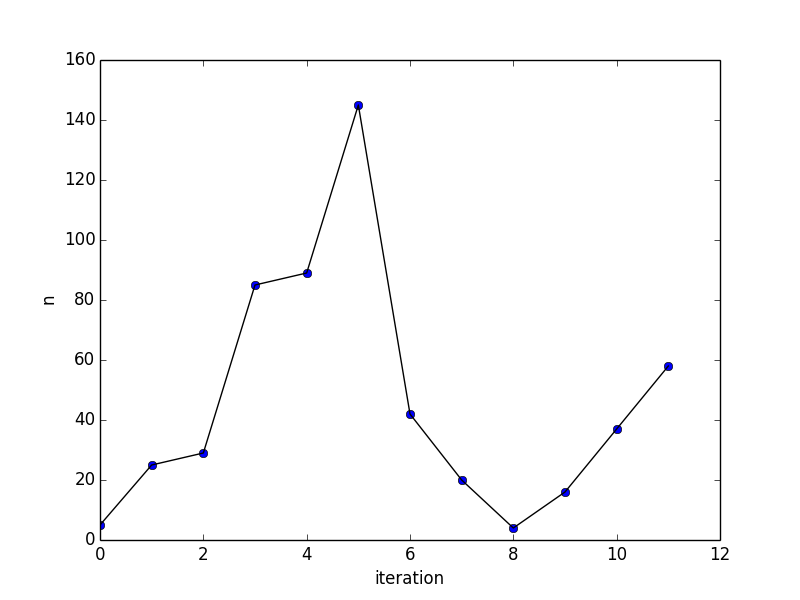
\includegraphics[width=.7\textwidth]{loop/happy_number.png}
    \caption{\label{fig:happy-number}The loop state, \code{n} \textit{vs.} iteration number.}
\end{figure}


This problem is relatively straightforward to solve.
In a loop, one keeps all the numbers discovered along the `path' along of the mapping from the
starting point.
When a number is detected to be repetition of an earlier one, terminate the loop.
Check if the terminating value of \code{n} is one.
A naïve implementation is as follows.
\lstinputlisting[label={lst:nonlinear-stepping},
caption={Dynamic stepping in a loop}]{loop/nonlinear_stepping_example.py}
The state of the loop is entirely encoded in the variable \code{n}.
The chart in ~\autoref{fig:happy-number} shows how the loop state changes as the program
executes for $n=7$.
Through this case, one can get a sense of how `dynamic' the pacing of a loop can be.


Trying different ways that a loop paces provides one more opportunity for it to best suit the
application.
This can be particularly helpful for `loop rotations' and compacting nested loops.
We will discuss more on this topic in ~\autoref{ch:loop-thinning}.


From the perspective of choice of loop constructs,
\code{while}-loop is more accommodating for all kinds of stepping.
for-loop, on the other hand, .
\code{for}-loop with niches for both initialization and the afterthought
statement, on the other hand, is built for steady pacing.
Unless it is for loop-variable isolation purposes, \code{for}-loop is not recommended for
dynamically paced construct.
On the other hand, if used \code{for}-loop in programs, tuning the pace of iteration may be as
simple as relocating the state-updating statements, \textit{e.g.},
from an afterthought statement to the loop body.
There is an unsaid convention regarding C-style \code{for}-loop---when the loop paces linearly
with a simple loop-state updating statement, it should be placed in the afterthought section of
the loop header.
Conversely, when you see the afterthought part missing, it should be a sign for dynamic
pacing.


\section{Conclusion}

The best practice when it comes to programming loops is to get a \emph{working version} (WV).
Once you get a WV, you can start to iterate for improvements:
duplicate code of any severity, excessive customization such as \code{break} or \code{continue}
\textit{etc}.
Try the techniques we talked about in this chapter such as `loop rotation',
`one-more-cycle', initialization reduction techniques, \textit{etc.}
Try on different loop constructs and so on.
Also keep in mind opportunities of using sentinels for certain niched applications (see
~\autoref{ch:sentinels}).
Finally, narrow down to a loop construct
that is a close match to your programming requirement
minimal loop customization, if needed at all.
The ultimate goal is to minimize or eliminate duplicate code in and around loop.

%\lstinputlisting[]{loop/NumberOfPath.java}
%\lstinputlisting[]{loop/WildcardStringMatching.java}
